\documentclass[12pt,a4paper]{article}
\usepackage[margin=1in]{geometry}
\usepackage[T1]{fontenc}
\usepackage{lmodern}
\usepackage{amsmath,amssymb,booktabs,array,tabularx}
\usepackage{graphicx,xcolor,float}
\usepackage{fancyhdr,enumitem,listings}
\usepackage{tikz,pgfplots}
\usetikzlibrary{arrows.meta,positioning,shapes.geometric}
\pgfplotsset{compat=1.18}
\usepackage[colorlinks=true,linkcolor=black,urlcolor=blue]{hyperref}
\hypersetup{pdftitle={Programming Assignment III: Learning to Rank},pdfauthor={search-o-SAURS}}
\setlength{\headheight}{15pt}
\pagestyle{fancy}
\fancyhf{}
\fancyhead[L]{\small search-o-SAURS}
\fancyhead[R]{\small Programming Assignment III}
\fancyfoot[C]{\thepage}
\setlength{\parindent}{0pt}
\setlength{\parskip}{4pt}
\setlist[itemize]{leftmargin=1.5em,itemsep=2pt,topsep=3pt}
\setlist[enumerate]{leftmargin=1.8em,itemsep=2pt,topsep=3pt}
\renewcommand{\arraystretch}{1.16}
\newcolumntype{Y}{>{\raggedright\arraybackslash}X}
\definecolor{zoneblue}{HTML}{4B538F}
\definecolor{svmteal}{HTML}{267C79}
\definecolor{paleblue}{HTML}{EAE9F5}
\lstset{basicstyle=\ttfamily\small,breaklines=true,columns=fullflexible,keepspaces=true,
  frame=single,rulecolor=\color{gray!45},xleftmargin=3pt,xrightmargin=3pt}
% Generated from actual PA3 outputs by prepare_report.py.
\newcommand{\CorpusTokens}{256,861}
\newcommand{\CorpusVocabulary}{9,422}
\newcommand{\AverageLength}{183.472}
\newcommand{\SelectedC}{0.1}
\newcommand{\RawIntercept}{-0.291903}
\newcommand{\ScaledIntercept}{-0.494632}
\newcommand{\BetterQueries}{29}
\newcommand{\TiedQueries}{13}
\newcommand{\WorseQueries}{3}
\newcommand{\ZoneZeroHits}{30}
\newcommand{\SvmZeroHits}{16}
\newcommand{\MaximumScoreError}{2.22e-15}
\newcommand{\SummaryRows}{%
A & Macro & 30 & 0.012593 & 0.075582 & 0.019683 & 17 / 1350 / 341 \\
A & Micro & 30 & 0.012593 & 0.049853 & 0.020106 & 17 / 1350 / 341 \\
B & Macro & 5 & 0.315556 & 0.260766 & 0.270154 & 71 / 225 / 341 \\
B & Micro & 5 & 0.315556 & 0.208211 & 0.250883 & 71 / 225 / 341 \\
}
\newcommand{\SplitRows}{%
Train & 135 & 189,000 & 991 & 188,009 \\
Validation & 45 & 63,000 & 280 & 62,720 \\
Test & 45 & 63,000 & 341 & 62,659 \\
}
\newcommand{\WeightRows}{%
$f_{1}$ & -0.0194058 & -0.135497 \\
$f_{2}$ & +0.463602 & +0.057099 \\
$f_{3}$ & -0.000115603 & -0.010393 \\
$f_{4}$ & -0.0564386 & -0.276684 \\
$f_{5}$ & -0.0114176 & -0.234726 \\
$f_{6}$ & +0.198982 & +0.001650 \\
$f_{7}$ & -0.0249545 & -0.231572 \\
$f_{8}$ & -0.057942 & -0.071641 \\
$f_{9}$ & +0.00804073 & +0.237202 \\
$f_{10}$ & +2.10505 & +0.166341 \\
$f_{11}$ & +45.9213 & +0.005458 \\
$f_{12}$ & +1.37187 & +0.045029 \\
$f_{13}$ & -52.5741 & -0.246634 \\
$f_{14}$ & +17.1219 & +0.005475 \\
$f_{15}$ & +0.00714147 & +0.175562 \\
$f_{16}$ & +1.39056 & +0.017122 \\
$f_{17}$ & -0.00102308 & -0.009392 \\
$f_{18}$ & +0.134272 & +0.196365 \\
$f_{19}$ & -0.00306328 & -0.095344 \\
$f_{20}$ & -7.75515 & -0.035677 \\
$f_{21}$ & +3.60034 & +0.152649 \\
$f_{22}$ & +0.135135 & +0.453768 \\
}
\newcommand{\ValidationRows}{%
0.01 & 5 & 0.241029 \\
0.1 & 5 & 0.247378 \\
1 & 5 & 0.247378 \\
}
\newcommand{\CutoffRows}{%
5 & 0.008889 & 0.006667 & 0.007407 & 0.315556 & 0.260766 & 0.270154 \\
10 & 0.011111 & 0.013006 & 0.011203 & 0.231111 & 0.368583 & 0.266222 \\
15 & 0.011852 & 0.021507 & 0.014601 & 0.188148 & 0.438903 & 0.245490 \\
20 & 0.010000 & 0.022815 & 0.013257 & 0.150000 & 0.457030 & 0.211795 \\
30 & 0.012593 & 0.075582 & 0.019683 & 0.112593 & 0.506284 & 0.174891 \\
}
\newcommand{\ExampleRows}{%
1 & 400 & 2.996310 & Relevant \\
2 & 1399 & 2.613746 & Unjudged \\
3 & 1387 & 1.879368 & Relevant \\
4 & 1400 & 1.874723 & Unjudged \\
5 & 1398 & 1.801843 & Relevant \\
}
\newcommand{\CurveA}{(5,0.00740741) (10,0.01120252) (15,0.01460148) (20,0.01325716) (30,0.01968314)}
\newcommand{\CurveB}{(5,0.27015366) (10,0.26622233) (15,0.24548967) (20,0.21179545) (30,0.17489081)}


\begin{document}
\hypersetup{pageanchor=false}
\begin{titlepage}
\centering
\vspace*{1.65cm}
{\Large\bfseries Information Retrieval\par}
\vspace{0.12cm}
{\large\bfseries Programming Assignment III\par}
\vspace{1.65cm}
{\LARGE\bfseries Learning to Rank Documents\par}
\vspace{0.3cm}
{\large\itshape on the Cranfield Aeronautics Corpus\par}
\vspace{1.5cm}
{\large\bfseries Group: search-o-SAURS\par}
\vspace{1.25cm}
\begin{tabular}{lr}
\toprule
\textbf{Name} & \textbf{Roll Number} \\
\midrule
Utsa Ghosh & \texttt{23CS10090} \\
Antariksh Das & \texttt{23CS10086} \\
Raktim Kundu & \texttt{23CS30044} \\
Souhardya Dandapat & \texttt{23CS30054} \\
Sharanya Baidya & \texttt{23CS30064} \\
\bottomrule
\end{tabular}
\vfill
{\bfseries Implementation, Experiments and Results\par}
\vspace{0.25cm}
{\small Boolean Weighted Zones and Linear Support Vector Machines\par}
\vspace*{0.9cm}
\end{titlepage}

\pagenumbering{arabic}
\hypersetup{pageanchor=true}
\tableofcontents
\clearpage

\section{Introduction}
This report describes the learning-to-rank system developed by group
\textbf{search-o-SAURS} for Programming Assignment III. The task is to order
Cranfield documents by their estimated relevance to a query, using the supplied
human relevance judgments to learn the ranking parameters.

Two methods are implemented. Method A learns four weights for Boolean matches
in the title, author, bibliography and text body. Method B learns a real-valued
linear score over the assignment's 22 query-document features using a support
vector machine (SVM). Both methods are evaluated on the same held-out queries
using precision, recall and F1. Saved weights also support new queries without
retraining.

\section{Assignment Requirements}
The programming requirements are addressed as follows:
\begin{enumerate}
\item Use the Cranfield collection and its provided relevance judgments.
\item Learn individual field weights for Boolean weighted zone scoring and use
      the weighted score to produce a ranked document list.
\item Train a \emph{linear} SVM using every feature listed in PA3.
\item Evaluate test-query result lists with precision, recall and F1.
\item Supply source programs, test rankings as text, and an implementation and
      experiment report; support further unknown test queries.
\end{enumerate}
PA3 permits SVM libraries and NLP tools. Only SVM fitting uses scikit-learn;
parsing, features, scaling, search, metrics, storage and tests use Python's
standard library. The statement does not fix feature formulas, preprocessing,
split proportions or retrieval cutoffs. Our choices are stated explicitly below.

\section{Dataset and Relevance Judgments}
\begin{table}[H]\centering\small
\caption{Statistics of the supplied collection after our tokenization.}
\begin{tabular}{lr}\toprule
Quantity & Value \\\midrule
Documents / queries & 1,400 / 225 \\
Judgments / positive judgments & 1,837 / 1,612 \\
Grade $-1$ judgments & 225 \\
Tokens / distinct vocabulary terms & \CorpusTokens{} / \CorpusVocabulary{} \\
Mean stream length / empty streams & \AverageLength{} / 2 \\
\bottomrule\end{tabular}\end{table}
Binary evaluation maps grades 1--4 to relevant and grade $-1$, 0, 5 or unjudged
pairs to nonrelevant. Document IDs are preserved. Qrels use a query's one-based
position in \texttt{cran.qry}, not its source \texttt{.I}: source IDs 1, 2, 4, 8
map to qrel IDs 1, 2, 3, 4.

\clearpage
\section{System Architecture and Preprocessing}
\begin{figure}[H]\centering
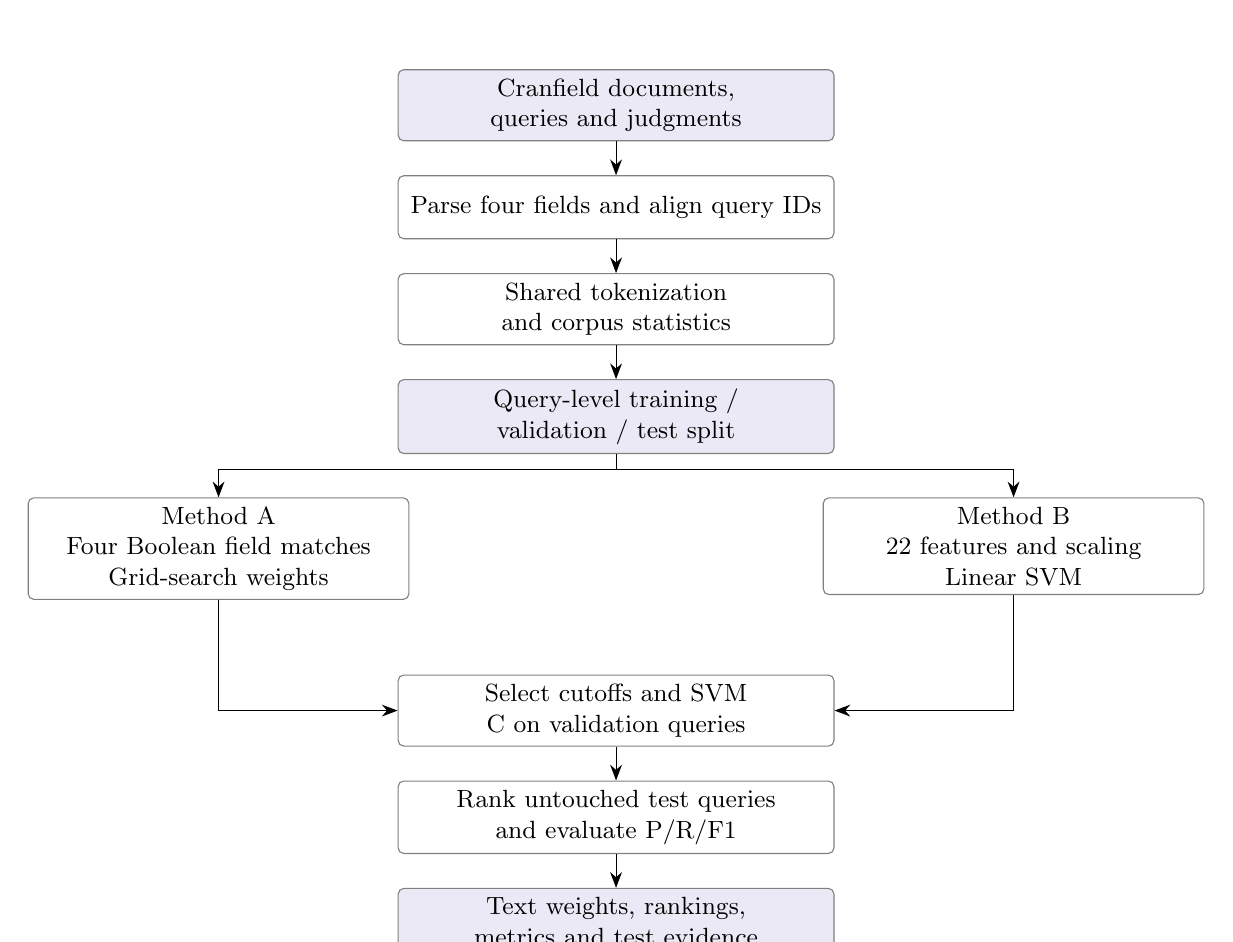
\begin{tikzpicture}[
  node distance=0.43cm and 0.55cm,
  box/.style={draw=gray,rounded corners=2pt,align=center,font=\small,
              minimum height=0.8cm,text width=5.3cm},
  smallbox/.style={box,text width=4.6cm},
  arrow/.style={-{Stealth[length=2mm]},thin}]
\node[box,fill=paleblue] (input) {Cranfield documents, queries and judgments};
\node[box,below=of input] (parse) {Parse four fields and align query IDs};
\node[box,below=of parse] (tokens) {Shared tokenization and corpus statistics};
\node[box,below=of tokens,fill=paleblue] (split) {Query-level training / validation / test split};
\node[smallbox,below left=0.55cm and -0.15cm of split] (zone) {Method A\\Four Boolean field matches\\Grid-search weights};
\node[smallbox,below right=0.55cm and -0.15cm of split] (svm) {Method B\\22 features and scaling\\Linear SVM};
\node[box,below=2.8cm of split] (select) {Select cutoffs and SVM C on validation queries};
\node[box,below=of select] (test) {Rank untouched test queries and evaluate P/R/F1};
\node[box,below=of test,fill=paleblue] (outputs) {Text weights, rankings, metrics and test evidence};
\draw[arrow] (input)--(parse);\draw[arrow] (parse)--(tokens);\draw[arrow] (tokens)--(split);
\draw[arrow] (split.south)--++(0,-0.2)-|(zone.north);
\draw[arrow] (split.south)--++(0,-0.2)-|(svm.north);
\draw[arrow] (zone.south)|-(select.west);\draw[arrow] (svm.south)|-(select.east);
\draw[arrow] (select)--(test);\draw[arrow] (test)--(outputs);
\end{tikzpicture}
\caption{Training and evaluation pipeline. Test labels never select parameters.}
\end{figure}
\begin{table}[H]\centering\small
\caption{Program responsibilities in the standalone source directory.}
\begin{tabularx}{\linewidth}{lY}\toprule
File in \texttt{src/} & Responsibility \\\midrule
\texttt{data.py} & Parse records, tokenize and build collection statistics. \\
\texttt{features.py} & Compute all 22 query-document features. \\
\texttt{zone\_model.py} & Learn and apply Boolean field weights. \\
\texttt{svm\_model.py} & Scale features, fit SVM and export coefficients. \\
\texttt{metrics.py} & Per-query, macro and micro precision/recall/F1. \\
\texttt{train.py}, \texttt{predict.py} & Run the experiment; apply saved models to new queries. \\
\bottomrule\end{tabularx}\end{table}
Tokenization lowercases text and extracts ASCII alphanumeric sequences. No
stemming, stopword removal or deduplication is applied; Method B retains
frequencies. Queries and fields use identical preprocessing. Repeated sections
are concatenated, and missing fields remain empty. The SVM defaults to all fields;
\texttt{--stream body} selects only the body. Empty queries return no results.

\clearpage
\section{Method A: Boolean Weighted Zone Scoring}
\subsection{Boolean Inputs and Ranking Score}
Let $Q$ contain the distinct processed query terms, and let $Z_z(d)$ be the term
set of document $d$ in zone $z$. For each of the four fields, default disjunctive
matching gives
\begin{equation}
 s_z(q,d)=\begin{cases}1,&Q\cap Z_z(d)\ne\varnothing,\\0,&\text{otherwise.}\end{cases}
 \qquad S_A(q,d)=\sum_{z\in\{T,A,B,W\}}w_zs_z(q,d).
\end{equation}
The constraints are $w_z\geq0$ and $\sum_z w_z=1$. Consequently scores lie in
$[0,1]$. An optional conjunctive mode requires every distinct query term to
occur in the same field; an empty query still scores zero. The reported experiment
uses disjunctive matching, as recorded in the saved parameters.

\subsection{Learning the Four Weights}
An exhaustive simplex grid uses weights in increments of $0.1$. Nonnegative
integer allocations $a+b+c+d=10$ yield
\[
 \binom{10+4-1}{4-1}=286
\]
candidate vectors. For each vector, the program ranks the training queries and
maximizes their mean per-query F1 at cutoff 10. An equal training score retains
the first enumerated vector. The learned weights are:
\begin{table}[H]\centering
\caption{Learned field weights from the 135 training queries.}
\begin{tabular}{lrrrr}\toprule
Field & Title & Author & Bibliography & Body \\\midrule
Weight & 0.3 & 0.1 & 0.2 & 0.4 \\
\bottomrule\end{tabular}\end{table}
Training macro F1 at 10 is $0.010520$. With weights fixed, validation queries
select the final cutoff from $\{5,10,15,20,30\}$. The selected cutoff is 30,
with validation macro F1 $0.005432$. The held-out test set is not consulted.

\subsection{Implementation and Ties}
Only 16 distinct four-field Boolean patterns exist. Grid evaluation caches results
only when pattern ordering, score ties and positive-score membership all agree.
This avoids repeated evaluation without changing the search objective. The tests
compare the optimized search with a separate exhaustive implementation over all
patterns, including ties and zero weights.

Zero scores are excluded. Grid sums are rounded to 12 places, and ties use
ascending document ID in training and inference alike. Common unfiltered terms
make many fields match, limiting discrimination; no secondary score conceals this.

\clearpage
\section{The 22 Query-Document Features}
For Method B, let $f_t=\mathrm{tf}(t,d)$, $L_d$ be document stream length and $N$
the document count. Define smoothed IDF and the query term frequency by
\[
 g_t=1+\ln\frac{N+1}{\mathrm{df}(t)+1},\qquad c_t=\mathrm{tf}(t,q).
\]
All term statistics below range over distinct query terms $Q$, including zeros for
absent terms. Write $\operatorname{stat}(v)$ for sum, minimum, maximum, mean and
population variance, in that order. This fixes the assignment's unspecified
statistical conventions.
\begin{table}[H]\centering\small
\caption{Complete feature vector, in assignment and implementation order.}
\begin{tabularx}{\linewidth}{r l Y}\toprule
No. & Feature & Definition \\\midrule
1 & Query term number & $\sum_{t\in Q}c_t$, including repeated query tokens. \\
2 & Query term ratio & $|\{t\in Q:f_t>0\}|/|Q|$. \\
3 & Stream length & $L_d$, counting all processed tokens. \\
4 & IDF & $\sum_{t\in Q:f_t>0}g_t$. \\
5 & TF sum & $\sum_{t\in Q} f_t$. \\
6 & TF minimum & $\min_{t\in Q} f_t$. \\
7 & TF maximum & $\max_{t\in Q} f_t$. \\
8 & TF mean & $|Q|^{-1}\sum_{t\in Q} f_t$. \\
9 & TF variance & $|Q|^{-1}\sum_{t\in Q}(f_t-\bar f)^2$. \\
10--14 & Normalized TF & $\operatorname{stat}(f_t/L_d)$. \\
15--19 & TF-IDF & $\operatorname{stat}(f_tg_t)$. \\
20 & Boolean model & 1 iff every distinct query term occurs in the stream. \\
21 & Vector space model & Cosine of raw-TF $\times$ smoothed-IDF vectors. \\
22 & BM25 & Saturated TF and length-normalized score below. \\
\bottomrule\end{tabularx}\end{table}
The VSM document norm uses the full document vocabulary, while the dot product
uses query terms. Query weights retain repetitions:
\[
 \operatorname{VSM}(q,d)=
 \frac{\sum_{t\in Q}(f_tg_t)(c_tg_t)}
 {\sqrt{\sum_{u\in d}(\mathrm{tf}(u,d)g_u)^2}
  \sqrt{\sum_{t\in Q}(c_tg_t)^2}}.
\]
BM25 sums once per distinct query term, with $k_1=1.2$, $b=0.75$:
\[
 \operatorname{BM25}(q,d)=\sum_{t\in Q}
 \ln\!\left(1+\frac{N-\mathrm{df}(t)+0.5}{\mathrm{df}(t)+0.5}\right)
 \frac{f_t(k_1+1)}{f_t+k_1(1-b+bL_d/\overline L)}.
\]
Zero-length streams have normalized TF zero; zero-norm cosine is zero. An unseen
term has $\mathrm{df}=0$ and document TF zero. Empty-query features are zero except
stream length, and the ranking API returns an empty result list. The default SVM
ranks all documents; a nonempty out-of-vocabulary query may still receive scores
through query-independent stream length. Lexical-only candidates are optional.

\clearpage
\section{Method B: Learning Real-Valued SVM Weights}
\subsection{Training and Exporting the Score}
Every training query is paired with all 1,400 documents. Positive judgments become
class 1; other pairs become class 0. Each feature is standardized using only the
training pairs: $z_j=(x_j-\mu_j)/\sigma_j$, with scale 1 for a constant feature.
The linear SVM uses balanced class weights, $\mathrm{dual}=\mathrm{False}$,
squared hinge loss and at most 20,000 iterations. A convergence warning fails the run.

In the margin formulation, labels are $y_i\in\{-1,+1\}$ and class weights are
$\alpha_y=n/(2n_y)$. With the default unit intercept scaling, the solver minimizes
\[
 \tfrac12(\|w'\|^2+(b')^2)+C\sum_i\alpha_{y_i}
       \max\{0,1-y_i(w'\!\cdot z_i+b')\}^2.
\]
For inference without sklearn, coefficients are converted to original units:
$w_j=w'_j/\sigma_j$ and $b=b'-\sum_jw_j\mu_j$. Documents are ranked by
$S_B(q,d)=w\cdot x(q,d)+b$, not predicted class labels. A negative score can
therefore appear in a selected top-$k$ list.

\begin{table}[H]\centering\small
\caption{Learned SVM coefficients. Feature numbers refer to Table 4.}
\setlength{\tabcolsep}{15pt}
\begin{tabular}{crr}\toprule
Feature & Original-unit $w_j$ & Standardized $w'_j$ \\\midrule
\WeightRows
\bottomrule\end{tabular}\end{table}
Selected $C=\SelectedC$; final cutoff $k=5$. Intercepts are $b=\RawIntercept$
and $b'=\ScaledIntercept$. Coefficient interpretation is discussed in Section 12.

\clearpage
\section{Plan of Experiments and Evaluation Measures}
\subsection{Query-Level Separation}
A local Python random generator with seed 42 shuffles sorted query IDs and assigns
60\% to training, 20\% to validation and 20\% to final testing. All query-document
pairs for one query stay together. The resulting label counts are:
\begin{table}[H]\centering\small
\caption{Experimental partitions and binary query-document labels.}
\begin{tabular}{lrrrr}\toprule
Partition & Queries & Pairs & Positive & Negative \\\midrule
\SplitRows
\bottomrule\end{tabular}\end{table}
The 991 positives among 189,000 training pairs explain the need for class
balancing. Validation selects operating settings only. Models are not refitted
after selection, so their saved coefficients reproduce the held-out predictions.
Corpus-wide IDF and average length are unsupervised statistics over the searchable
collection, not statistics learned from test labels.

\subsection{Settings and Selection Procedure}
Method A searches 286 vectors using training macro F1 at 10, then chooses a
validation cutoff. Method B tries $C\in\{0.01,0.1,1\}$ and the same five cutoffs.
Its best validation result at each C is shown below; the tie between 0.1 and 1
selects 0.1. Cutoff ties select the smaller value.
\begin{table}[H]\centering\small
\caption{Validation selection for the pointwise linear SVM.}
\begin{tabular}{rrr}\toprule
$C$ & Best cutoff & Validation macro F1 \\\midrule
\ValidationRows
\bottomrule\end{tabular}\end{table}

\subsection{Precision, Recall and F1}
Let $R_q$ be the actually returned list and $G_q$ the known relevant document set.
With $h_q=|R_q\cap G_q|$,
\[
 P_q=\frac{h_q}{|R_q|},\qquad R_q^{\mathrm{metric}}=\frac{h_q}{|G_q|},\qquad
 F1_q=\frac{2P_qR_q^{\mathrm{metric}}}{P_q+R_q^{\mathrm{metric}}}.
\]
Empty denominators give zero. Precision uses the actual returned count. Macro
scores average per-query values, including zero-hit queries; macro F1 averages
query F1. Micro scores pool hit, retrieved and relevant counts. All measurements
use the exact exported lists.

\clearpage
\section{Held-Out Results}
\subsection{Primary Test Evaluation}
The following results use each model's validation-selected cutoff on the same 45
untouched test queries. The test set contains 341 positive judgments. Full
per-query measurements are supplied in \texttt{results/evaluation.txt}.
\begin{table}[H]\centering\scriptsize
\caption{Primary test results. H/Ret/Rel denotes pooled hits/retrieved/relevant counts.}
\setlength{\tabcolsep}{4pt}
\begin{tabular}{llrrrrl}\toprule
Method & Average & $k$ & Precision & Recall & F1 & H / Ret / Rel \\\midrule
\SummaryRows
\bottomrule\end{tabular}\end{table}

\begin{figure}[H]\centering
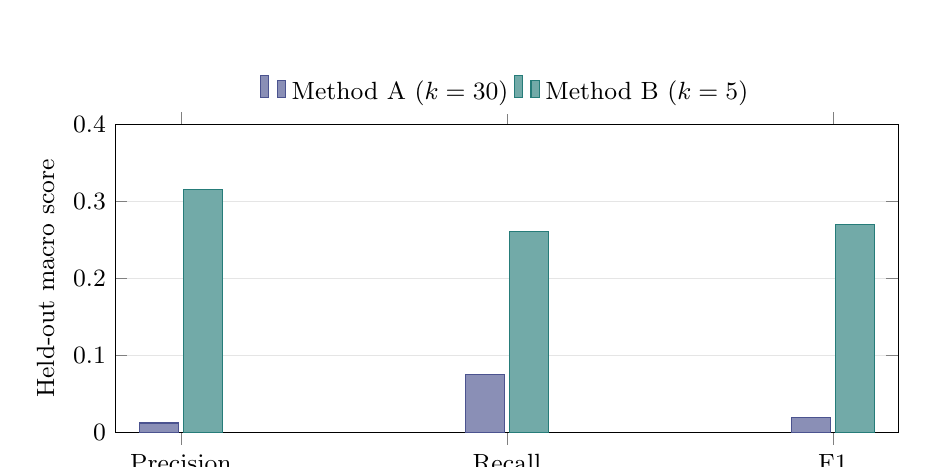
\begin{tikzpicture}
\begin{axis}[width=0.95\linewidth,height=5.5cm,ybar,bar width=14pt,
  ymin=0,ymax=0.40,ylabel={Held-out macro score},
  symbolic x coords={Precision,Recall,F1},xtick=data,
  ymajorgrids=true,grid style={gray!20},
  legend style={at={(0.5,1.03)},anchor=south,legend columns=2,draw=none,font=\small},
  tick label style={font=\small},label style={font=\small}]
\addplot[fill=zoneblue!65,draw=zoneblue] coordinates {(Precision,0.0125925926) (Recall,0.0755821738) (F1,0.0196831439)};
\addplot[fill=svmteal!65,draw=svmteal] coordinates {(Precision,0.3155555556) (Recall,0.2607662862) (F1,0.2701536607)};
\legend{Method A ($k=30$),Method B ($k=5$)}
\end{axis}
\end{tikzpicture}
\caption{Macro metrics at the operating points selected on validation queries.}
\end{figure}
Method B retrieves 71 judged relevant documents in 225 returned positions, while
Method A retrieves 17 in 1,350 positions. Method B has higher precision and recall
despite returning shorter lists. The differing cutoffs mean this is an
operating-point comparison; Section 10 also compares identical cutoffs.

There are \ZoneZeroHits{} zero-hit queries for Method A and \SvmZeroHits{} for Method B.
On per-query F1, Method B is better on \BetterQueries{} queries, tied on
\TiedQueries{} and worse on \WorseQueries{}. These are descriptive results from one
split, not a statistical significance claim. The difference between macro and
micro recall also shows that the per-query relevant-set sizes are unequal.

\clearpage
\section{Cutoff Analysis and a Query Example}
This additional analysis fixes the already learned models and evaluates the test
queries at common cutoffs. It does not retrain the models or use these test results
to revise their selected operating points.
\begin{table}[H]\centering\scriptsize
\caption{Held-out macro metrics at identical cutoffs, using fixed learned weights.}
\setlength{\tabcolsep}{5pt}
\begin{tabular}{rrrrrrr}\toprule
& \multicolumn{3}{c}{Method A} & \multicolumn{3}{c}{Method B} \\
$k$ & P & R & F1 & P & R & F1 \\\midrule
\CutoffRows
\bottomrule\end{tabular}\end{table}
\begin{figure}[H]\centering
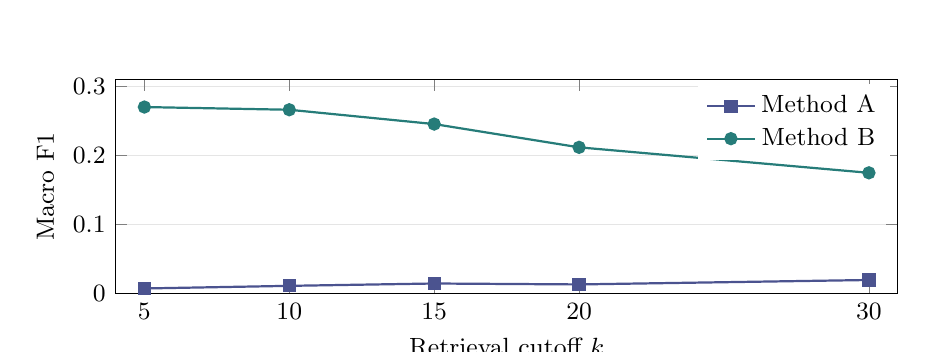
\begin{tikzpicture}
\begin{axis}[width=0.95\linewidth,height=4.3cm,xlabel={Retrieval cutoff $k$},ylabel={Macro F1},
  xmin=4,xmax=31,ymin=0,ymax=0.31,xtick={5,10,15,20,30},
  ymajorgrids=true,grid style={gray!20},
  legend style={at={(0.99,0.98)},anchor=north east,draw=none,font=\small},
  tick label style={font=\small},label style={font=\small}]
\addplot[color=zoneblue,mark=square*,thick] coordinates {\CurveA};
\addplot[color=svmteal,mark=*,thick] coordinates {\CurveB};
\legend{Method A,Method B}
\end{axis}
\end{tikzpicture}
\caption{The SVM advantage persists when cutoff size is controlled.}
\end{figure}
At larger SVM cutoffs, recall rises but precision and F1 fall. Method A remains
weak at every tested cutoff, consistent with its coarse Boolean inputs and many
ties. No BM25 baseline or alternative preprocessing experiment was run here;
their effects cannot be inferred from these measurements.

For query 223 (source ID 356), \emph{``papers on shear buckling of unstiffened
rectangular plates under shear''}, the five SVM results are:
\begin{table}[H]\centering\small
\caption{Example SVM output, evaluated using supplied judgments only.}
\begin{tabular}{rrrl}\toprule
Rank & Document & Score & Judgment \\\midrule
\ExampleRows
\bottomrule\end{tabular}\end{table}
Three hits among five results and four known relevant documents give
$P=0.6$, $R=0.75$, $F1=2/3$. ``Unjudged'' means absent from the positive qrels;
the evaluation treats it as nonrelevant without asserting its true semantic relevance.

\clearpage
\section{Testing, Validation and Complexity}
The standard-library test suite contains \textbf{33 tests}, with zero failures,
errors or skips in the final run. It checks computation and output correctness
separately from retrieval effectiveness.
\begin{table}[H]\centering\small
\caption{Validation evidence recorded in the submitted test reports.}
\begin{tabularx}{\linewidth}{>{\raggedright\arraybackslash}p{3.5cm}Y}\toprule
Check & Evidence \\\midrule
Parsing and data integrity & Independent reader matches all 1,400 records; repeated fields retained; ordinal query alignment and grade counts verified. \\
Feature calculations & 35,200 values checked independently: 25 documents, 32 queries, two stream choices and 22 features. \\
Zone learning & Cached grid search equals exhaustive evaluation for grid divisions 2, 3 and 10, including all Boolean patterns and ties. \\
SVM mathematics & Exported scores agree with the solver's own decision function; non-unit scaling and intercept conversion tested. \\
Real outputs & All 45 test queries scored across 1,400 documents; saved rankings and all P/R/F1 values independently checked. \\
Data isolation & Altering only final-test labels leaves learned parameters, selected cutoffs and ranking files unchanged. \\
Inference and repeatability & CLI works with site-packages disabled; fresh full training reproduces all eight experiment files byte-for-byte. \\
\bottomrule\end{tabularx}\end{table}
The largest recorded discrepancy between standardized-coordinate SVM scores and
exported original-unit scores is $2.22\times10^{-15}$, consistent with floating-point
rounding. The source dataset's hashes remain unchanged during testing. Test outputs
are in \path{test_results.txt}, \path{output_verification.txt} and
\path{retraining_test.txt} under \texttt{results/}.

For $D$ documents, $m$ distinct query terms and $p=22$ features, feature extraction
is $O(Dm)$ after corpus statistics are available. A linear scoring pass is $O(Dp)$;
sorting is $O(D\log D)$. Zone grid search has 286 candidates and training-query
ranking work in the worst case; caching equivalent orderings reduces repeated work.
SVM optimization cost depends on the solver and data, so no fixed iteration count
or training-time speedup is claimed.

The experiment caches $225\times1{,}400\times22=6{,}930{,}000$ feature values,
plus standardized training rows and corpus statistics. This is a count of values,
not a claim that Python object storage occupies only a dense float-array size.

\clearpage
\section{Discussion, Deliverables and Conclusion}
\subsection{What the Results Establish}
The linear SVM is substantially more effective than the learned Boolean zones on
this held-out split, including at identical cutoffs. Query coverage, frequencies,
length normalization, VSM and BM25 provide distinctions absent from four field bits.
The learned Boolean weights emphasize body and title, but many documents share
the same Boolean pattern. Ascending-ID ties make this limitation reproducible
rather than concealing it with an extra retrieval signal.

Large original-unit normalized-TF coefficients reflect small feature scales;
they do not establish that these features are intrinsically more important.
The negative AND-feature coefficient is learned from rare joint matches and
correlated inputs, not a general recommendation to penalize complete query coverage.
The pointwise SVM optimizes classification margins, while model selection uses
ranking-list F1; no pairwise ranking loss is claimed.

The evaluation is limited to one deterministic split and the supplied judgments.
Binary conversion discards graded distinctions and treats unjudged pairs as
negative. No significance test, external query evaluation, cross-validation study
or guarantee of future-query performance is reported. Possible later experiments
include stopword handling, term-level zone coverage and pairwise SVM training,
but these have not been measured in this submission.

\subsection{Files and Reproduction}
The deliverables are the programs in \texttt{src/}, tests in \texttt{tests/}, this
report, and the text files in \texttt{results/}. The two required ranking files are
\path{results_method_a.txt} and \path{results_method_b.txt}. Each line is
\texttt{query\_id Q0 document\_id rank score run\_tag}. The evaluated cutoff is
recorded separately; result lines use exactly that cutoff.
\begin{lstlisting}
python -m pip install -r requirements.txt
python src/train.py
python -B tests/run_tests.py --retrain
python src/predict.py --method svm --query "heat" --output search.txt
\end{lstlisting}
\texttt{weights.txt} stores field weights, all 22 SVM coefficients, intercept,
scaling parameters and configuration as Python literal data. Prediction loads it
with \texttt{ast.literal\_eval}; there is no JSON or binary model dependency.
External queries may be Cranfield records, ID-tab-text rows or plain lines.
Source IDs are preserved by default; \texttt{--query-id-mode ordinal} aligns the
original Cranfield query file to its judgments.

\subsection{Conclusion}
Both required methods, all 22 features, ranked outputs and precision/recall/F1 are
implemented and independently checked. The SVM's macro F1 is 0.270154 versus
0.019683 for Boolean zones. These measure retrieval quality, not correctness-test
pass rates; unspecified implementation choices are documented explicitly.

\end{document}
